\documentclass[aspectratio=169,11pt]{beamer}
% =====================================================================
%  Le Collé — thème de présentation (même palette et mêmes notations que la fiche)
% =====================================================================
\usepackage[utf8]{inputenc}
\usepackage[T1]{fontenc}
\usepackage[sc]{mathpazo}
\usepackage[scaled=0.92]{helvet}
\usefonttheme{professionalfonts}
\usepackage{amsmath,amssymb,mathrsfs,stmaryrd}
\usepackage{microtype}
\usepackage{booktabs,array,multicol}
\usepackage[most]{tcolorbox}
\usepackage{tikz,pgfplots}
\usetikzlibrary{arrows.meta,calc,positioning,decorations.pathreplacing,shapes.misc}
\pgfplotsset{compat=1.17,trig format plots=rad}
\usepackage{tkz-tab}

% ---------- palette (identique à la fiche) ----------
\definecolor{Ink}{HTML}{1C2533}\definecolor{Bleu}{HTML}{1F3A5F}\definecolor{BleuMoyen}{HTML}{4A6A8F}
\definecolor{BleuClair}{HTML}{9DB2C9}\definecolor{Fond}{HTML}{F2F4F7}\definecolor{Ocre}{HTML}{B07A26}
\definecolor{Brique}{HTML}{A23B2A}\definecolor{Gris}{HTML}{5E6672}\definecolor{Filet}{HTML}{C5CCD6}
\definecolor{Vert}{HTML}{2E6B4F}

% ---------- notations (identiques à la fiche) ----------
\newcommand{\K}{\mathbb{K}}\newcommand{\R}{\mathbb{R}}\newcommand{\C}{\mathbb{C}}\newcommand{\Z}{\mathbb{Z}}
\newcommand{\Mn}[1]{\mathcal{M}_{n}(#1)}\newcommand{\rg}{\operatorname{rg}}\newcommand{\vect}{\operatorname{Vect}}
\newcommand{\Mat}{\operatorname{Mat}}\newcommand{\Id}{\operatorname{Id}}\newcommand{\com}{\operatorname{com}}
\newcommand{\vv}[1]{\overrightarrow{#1}}\newcommand{\ve}[1]{\vec{#1}}
\newcommand{\dt}[1]{\left|\begin{matrix}#1\end{matrix}\right|}
\DeclareRobustCommand{\HP}{{\sffamily\bfseries\scriptsize\textcolor{Brique}{[HP]}}}

% ---------- réglages beamer ----------
\setbeamertemplate{navigation symbols}{}
\setbeamersize{text margin left=0.85cm,text margin right=0.85cm}
\setbeamercolor{normal text}{fg=Ink,bg=white}
\setbeamercolor{structure}{fg=Bleu}
\setbeamercolor{alerted text}{fg=Brique}
\setbeamerfont{alerted text}{series=\bfseries}
\setbeamertemplate{itemize item}{\raisebox{0.15em}{\textcolor{Ocre}{\rule{0.38em}{0.38em}}}}
\setbeamertemplate{itemize subitem}{\textcolor{BleuMoyen}{\scriptsize\textbullet}}
\setbeamertemplate{enumerate item}{\textcolor{Bleu}{\sffamily\bfseries\insertenumlabel.}}
\setlength{\leftmargini}{1.2em}
\setbeamertemplate{blocks}[default]

% numéro de la partie courante, rappelé dans le titre et le pied de page (renvoi à la fiche)
\def\fichesec{}\def\chapnom{}
\newcommand{\chapitre}[1]{\def\chapnom{#1}}

\setbeamertemplate{frametitle}{%
  \vskip0.28cm
  \ifx\fichesec\empty\else
    \tikz[baseline=(b.base)]\node[fill=Ocre,text=white,font=\sffamily\bfseries\scriptsize,inner sep=2.5pt,rounded corners=1pt](b){\fichesec};\hspace{0.45em}%
  \fi
  {\color{Bleu}\sffamily\bfseries\Large\insertframetitle}\par
  \vskip0.06cm{\color{Filet}\rule{\linewidth}{0.5pt}}\vskip-0.2cm}

\setbeamertemplate{footline}{%
  \hbox to\paperwidth{%
    \hspace*{0.85cm}{\scriptsize\sffamily\color{Gris}Le Collé\ \ \textcolor{Filet}{|}\ \ \chapnom}\hfill
    {\scriptsize\sffamily\color{Gris}\ifx\fichesec\empty\else fiche \textbf{\color{Ocre}§\fichesec}\quad\fi\insertframenumber}\hspace*{0.85cm}}%
  \vskip0.18cm
  \hbox{\begin{tikzpicture}
    \fill[Fond] (0,0) rectangle (\paperwidth,2.2pt);
    \pgfmathsetmacro\prog{min(\insertframenumber/max(\inserttotalframenumber,1),1)}
    \fill[Ocre] (0,0) rectangle ({\prog*\paperwidth},2.2pt);
  \end{tikzpicture}}}

% ---------- encadrés : même code couleur que la fiche ----------
\tcbset{sb/.style={enhanced,arc=1pt,boxrule=0pt,left=6pt,right=6pt,top=3pt,bottom=3pt,before skip=0.14cm,after skip=0.14cm,
  fontupper=\normalsize\raggedright}}
\newcommand{\etiq}[2]{{\sffamily\bfseries\scriptsize\color{#1}\MakeUppercase{#2}}\par\vspace{2pt}}
\newtcolorbox{DEF}[1][Définition]{sb,colback=white,borderline west={2pt}{0pt}{Bleu},before upper={\etiq{Bleu}{#1}}}
\newtcolorbox{PROP}[1][Propriété]{sb,colback=Fond,borderline west={3pt}{0pt}{Bleu},before upper={\etiq{Bleu}{#1}}}
\newtcolorbox{FORM}[1][Formule]{sb,colback=white,colframe=BleuMoyen,boxrule=0.6pt,before upper={\etiq{BleuMoyen}{#1}}}
\newtcolorbox{METH}[1]{sb,colback=white,borderline north={1pt}{0pt}{Bleu},borderline south={1pt}{0pt}{Bleu},
  before upper={{\sffamily\bfseries\scriptsize\colorbox{Bleu}{\color{white}MÉTHODE}\ \color{Bleu}#1}\par\vspace{3pt}}}
\newtcolorbox{PIEGE}[1][Piège]{sb,colback=Brique!6,borderline west={2pt}{0pt}{Brique},before upper={\etiq{Brique}{#1}}}
\newtcolorbox{ASTU}[1][Astuce]{sb,colback=Ocre!8,borderline west={2pt}{0pt}{Ocre},before upper={\etiq{Ocre}{#1}}}
\newtcolorbox{HPBOX}{sb,colback=white,borderline west={2pt}{0pt}{Brique},before upper={\etiq{Brique}{Hors programme}}}
\newtcolorbox{ATOI}[1][À toi]{sb,colback=Vert!6,borderline west={2pt}{0pt}{Vert},before upper={\etiq{Vert}{#1}}}
\newtcolorbox{RETENIR}{sb,colback=Bleu!5,colframe=Bleu,boxrule=0.8pt,left=8pt,
  before upper={\etiq{Bleu}{À retenir}}}
\newtcolorbox{EX}[1][Exemple]{sb,colback=white,colframe=Filet,boxrule=0.5pt,before upper={\etiq{Gris}{#1}}}

% complément pédagogique absent du livre : étiquette pointillée
\DeclareRobustCommand{\ajout}{\tikz[baseline=(a.base)]\node[draw=Gris,dashed,text=Gris,font=\sffamily\scriptsize,inner sep=2pt,rounded corners=1pt](a){complément hors livre};}
\newcommand{\livre}[1]{{\sffamily\scriptsize\color{Gris}[livre #1]}}
\newcommand{\rep}[1]{\textcolor{Vert}{#1}}% réponse attendue de l'élève

% ---------- styles de figures (identiques au livre) ----------
\pgfplotsset{courbe/.style={axis lines=middle,axis equal image,
  axis line style={Gris,-{Stealth[length=4pt]}},
  xlabel={$x$},ylabel={$y$},ticklabel style={font=\scriptsize\sffamily,color=Gris},
  every axis x label/.style={at={(ticklabel* cs:1)},anchor=west,font=\small},
  every axis y label/.style={at={(ticklabel* cs:1)},anchor=south,font=\small},
  samples=200,smooth}}
\pgfplotsset{mini/.style={axis lines=middle,axis line style={Filet},xtick=\empty,ytick=\empty,width=3.9cm,height=3.9cm,
  xmin=-1.15,xmax=1.15,ymin=-1.15,ymax=1.15,title style={font=\footnotesize\sffamily,yshift=-0.1cm},samples=100}}
\tikzset{arcetude/.style={Bleu,line width=1.25pt},
         reste/.style={BleuClair,line width=1pt},
         tgte/.style={Ocre,line width=1pt},
         asy/.style={Gris,dashed,line width=0.7pt},
         pt/.style={circle,fill=Ink,inner sep=1.3pt},
         >={Stealth[length=5pt]}}

% ---------- diapositives de partie ----------
% \partie{num}{titre}{question guide}{liste des parties du chapitre via \rm}
\newcommand{\rmitem}[2]{\def\tmp{#1}%
  \ifx\tmp\fichesec{\color{Bleu}\bfseries #1\quad #2}\else{\color{Gris!70}#1\quad #2}\fi\par\vspace{2pt}}
\newcommand{\partie}[4]{%
  \def\fichesec{#1}\section{#2}%
  \begin{frame}[plain]
  \begin{tikzpicture}[remember picture,overlay]
    \fill[Bleu] (current page.north west) rectangle ([xshift=6.3cm]current page.south west);
    \node[anchor=north west,text=white,font=\sffamily\bfseries\fontsize{40}{40}\selectfont] at ([xshift=0.8cm,yshift=-1.2cm]current page.north west) {#1};
    \node[anchor=north west,text width=4.8cm,align=left,text=white,font=\sffamily\bfseries\Large] at ([xshift=0.8cm,yshift=-2.9cm]current page.north west) {\hyphenpenalty=10000\exhyphenpenalty=10000 #2\par};
    \node[anchor=south west,text width=4.8cm,text=white!75!Bleu,font=\sffamily\scriptsize] at ([xshift=0.8cm,yshift=0.6cm]current page.south west) {\chapnom\\fiche \textbf{§#1}};
  \end{tikzpicture}
  \hspace*{5.5cm}\begin{minipage}{8.4cm}
  {\sffamily\scriptsize\color{Ocre}\bfseries LA QUESTION}\par\vspace{2pt}
  {\large #3}\par\vspace{0.7cm}
  {\sffamily\scriptsize\color{Gris}\bfseries DANS CE CHAPITRE}\par\vspace{4pt}
  {\sffamily\small #4}
  \end{minipage}
  \end{frame}}


% ---------- exercices en séance : énoncé sur une diapositive, correction sur la suivante ----------
\newcommand{\badgeexo}[1]{\tikz[baseline=(e.base)]\node[fill=Vert,text=white,font=\sffamily\bfseries\scriptsize,inner sep=2.5pt,rounded corners=1pt](e){EXERCICE #1};\hspace{0.4em}}
\newcommand{\badgecor}[1]{\tikz[baseline=(e.base)]\node[draw=Vert,line width=0.8pt,text=Vert,font=\sffamily\bfseries\scriptsize,inner sep=2.2pt,rounded corners=1pt](e){CORRECTION #1};\hspace{0.4em}}
\newtcolorbox{ENONCE}[1][]{sb,colback=Vert!6,borderline west={3pt}{0pt}{Vert},left=9pt,top=5pt,bottom=5pt,
  before upper={{\sffamily\bfseries\scriptsize\color{Vert}À TOI\ifx\relax#1\relax\else\ \ ·\ \ \MakeUppercase{#1}\fi}\par\vspace{4pt}}}
\newtcolorbox{INDICE}{sb,colback=white,colframe=Vert!60,boxrule=0.5pt,before upper={\etiq{Vert}{Indice (si besoin)}}}
\newtcolorbox{RAIS}[1][Le raisonnement]{sb,colback=Vert!5,borderline west={2pt}{0pt}{Vert},before upper={\etiq{Vert}{#1}}}
\newtcolorbox{OUTIL}{sb,colback=Fond,borderline west={2pt}{0pt}{Bleu},before upper={\etiq{Bleu}{Propriété ou méthode utilisée}}}
\newcommand{\etape}[1]{{\sffamily\bfseries\footnotesize\color{Vert}#1}\ }
\newcommand{\objectif}[1]{\par\vspace{2pt}{\footnotesize\sffamily\color{Gris}Objectif : #1}}

\title{Le Collé --- Courbes paramétrées planes}

\begin{document}

% ---------------------------------------------------------------- titre
\begin{frame}[plain]
\begin{tikzpicture}[remember picture,overlay]
  \fill[Bleu] (current page.north west) rectangle (current page.south east);
  \node[anchor=north west,text=white!70!Bleu,font=\sffamily\scriptsize] at ([xshift=1cm,yshift=-1.2cm]current page.north west)
    {LE COLLÉ\ \ ·\ \ MATHÉMATIQUES PT\ \ ·\ \ CHAPITRE 5\ \ ·\ \ SUPPORT DE SÉANCE};
  \node[anchor=north west,text=white,font=\sffamily\bfseries\fontsize{26}{30}\selectfont,text width=13cm] at ([xshift=1cm,yshift=-2.1cm]current page.north west)
    {Courbes paramétrées\\ planes};
  \fill[Ocre] ([xshift=1cm,yshift=-4.6cm]current page.north west) rectangle ([xshift=4cm,yshift=-4.65cm]current page.north west);
  \node[anchor=north west,text=white!80!Bleu,font=\normalsize,text width=12cm] at ([xshift=1cm,yshift=-5cm]current page.north west)
    {Présentation pour expliquer, avec quatre exercices à chercher en séance ; le \textbf{livret} pour relire, la \textbf{fiche} pour réviser.\\
     Mêmes parties (§2.1 à §2.7), mêmes notations, mêmes énoncés.};
\end{tikzpicture}
\end{frame}

% ---------------------------------------------------------------- mode d'emploi
\begin{frame}{Comment lire ce support}
\vspace{-0.15cm}
\begin{columns}[T]
\column{0.48\textwidth}
\begin{DEF}vocabulaire à connaître\end{DEF}\vspace{-9pt}
\begin{PROP}[Propriété / théorème]énoncé précis, avec ses hypothèses\end{PROP}\vspace{-9pt}
\begin{FORM}formule et conditions d'emploi\end{FORM}\vspace{-9pt}
\begin{METH}{}démarche à suivre, étape par étape\end{METH}
\column{0.48\textwidth}
\begin{PIEGE}erreur classique à éviter\end{PIEGE}\vspace{-9pt}
\begin{ASTU}technique qui fait gagner du temps\end{ASTU}\vspace{-9pt}
\begin{ATOI}question ou exercice ; correction à la diapositive suivante\end{ATOI}\vspace{-9pt}
\begin{RETENIR}l'essentiel d'une partie\end{RETENIR}
\end{columns}
{\footnotesize Même code couleur que la fiche. \ajout{} : ajout absent du livre. \ \HP{} : hors programme.
\ Le numéro ocre \tikz[baseline=(b.base)]\node[fill=Ocre,text=white,font=\sffamily\bfseries\scriptsize,inner sep=2pt](b){1.2};
\ renvoie à la partie de la fiche.}
\end{frame}

% ---------------------------------------------------------------- plan
\begin{frame}{Plan et séances}
\begin{columns}[T]
\column{0.54\textwidth}
{\sffamily\bfseries\color{Bleu}Chapitre 5 --- Courbes paramétrées}\par\vspace{4pt}
\small
2.1\quad Fonctions vectorielles, outils de calcul\\
2.2\quad Tangente, pente \hfill{\color{Vert}Ex.~1}\\
2.3\quad Plan d'étude, symétries, tracé \hfill{\color{Vert}Ex.~2}\\
2.4\quad Points stationnaires, étude locale, inflexions \hfill{\color{Vert}Ex.~3}\\
2.5\quad Branches infinies, positions \hfill{\color{Vert}Ex.~4}\\
2.6\quad Intersections, points doubles\\
2.7\quad Check-list et résultats des TD
\column{0.4\textwidth}
\begin{ASTU}[Découpage suggéré]
\small Séance 1 : 2.1--2.3\\ Séance 2 : 2.4--2.7, puis TD\hfill\ajout
\end{ASTU}
{\small\color{Gris}Les numéros §2.1 à §2.7 sont ceux du livret et de la fiche.}
\end{columns}
\end{frame}

% =====================================================================
%                CHAPITRE 2 — COURBES PARAMÉTRÉES PLANES
% =====================================================================
\chapitre{Chapitre 5 · Courbes paramétrées planes}
\def\fichesec{}
\newcommand{\rmII}{\rmitem{2.1}{Fonctions vectorielles, outils de calcul}\rmitem{2.2}{Tangente, pente}\rmitem{2.3}{Plan d'étude, symétries, tracé}
  \rmitem{2.4}{Points stationnaires, étude locale, inflexions}\rmitem{2.5}{Branches infinies, positions}\rmitem{2.6}{Intersections, points doubles}
  \rmitem{2.7}{Check-list et résultats des TD}}

\begin{frame}[plain]
\begin{tikzpicture}[remember picture,overlay]
  \fill[Bleu] (current page.north west) rectangle (current page.south east);
  \fill[Ocre] ([yshift=-4.2cm]current page.north west) rectangle ([yshift=-4.25cm,xshift=5cm]current page.north west);
  \node[anchor=north west,text=white!70!Bleu,font=\sffamily\small] at ([xshift=1cm,yshift=-1.6cm]current page.north west) {Chapitre 5};
  \node[anchor=north west,text=white,font=\sffamily\bfseries\fontsize{28}{30}\selectfont] at ([xshift=1cm,yshift=-2.3cm]current page.north west) {Courbes paramétrées};
  \node[anchor=north west,text width=8.5cm,text=white,font=\large] at ([xshift=1cm,yshift=-4.7cm]current page.north west)
    {Décrire une courbe par un point mobile $M(t)$.\\[2pt]
     \normalsize\color{white!75!Bleu} Étudier une courbe, c'est savoir la tracer avec ses points remarquables, ses tangentes et ses
     branches infinies.};
  \begin{axis}[at={([xshift=-5.3cm,yshift=-7.6cm]current page.north east)},anchor=south west,width=4.6cm,height=6.6cm,hide axis,
     xmin=-1.3,xmax=1.3,ymin=-2.3,ymax=2.3,samples=300,smooth]
   \addplot[white,line width=1.4pt,domain=0:6.2832]({cos(3*x)},{2*sin(x)});
  \end{axis}
\end{tikzpicture}
\end{frame}

% =====================================================================
\partie{2.1}{Fonctions vectorielles, outils de calcul}{Pourquoi décrire une courbe par $t\mapsto M(t)$ plutôt que par $y=g(x)$ ?}{\rmII}

\begin{frame}{Quand $y=g(x)$ ne suffit plus}
\begin{columns}[c]
\column{0.55\textwidth}
Un cercle, une boucle : à une abscisse correspondent \alert{plusieurs points}. On décrit alors la courbe par un \textbf{point
mobile}.
\pause
\begin{DEF}
Courbe paramétrée : $f:I\to\R^2$ (ou $\R^3$) de classe $\mathcal C^1$,
\[f(t)=\vv{OM(t)}=\big(x(t),y(t)\big).\]
Support : $\{M(t),\ t\in I\}$.
\end{DEF}
\pause
Équation cartésienne $F(x,y)=0$ $\neq$ représentation paramétrique.
\column{0.4\textwidth}\centering\onslide<1->
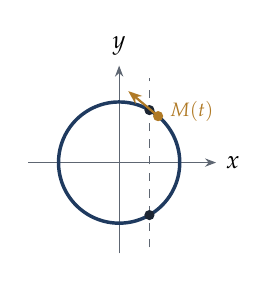
\begin{tikzpicture}
\begin{axis}[courbe,width=4.6cm,xmin=-1.5,xmax=1.6,ymin=-1.5,ymax=1.6,xtick=\empty,ytick=\empty]
\addplot[arcetude,domain=0:6.2832]({cos(x)},{sin(x)});
\draw[Gris,dashed] (axis cs:0.5,-1.4)--(axis cs:0.5,1.4);
\node[pt] at (axis cs:0.5,0.866) {}; \node[pt] at (axis cs:0.5,-0.866) {};
\node[pt,fill=Ocre] at (axis cs:0.643,0.766) {};
\draw[->,Ocre,thick] (axis cs:0.643,0.766)--(axis cs:0.15,1.18);
\node[font=\scriptsize,Ocre,anchor=west] at (axis cs:0.68,0.85) {$M(t)$};
\end{axis}
\end{tikzpicture}\\
{\scriptsize deux points pour la même abscisse ;\\ le point $M(t)$ et sa vitesse}
\end{columns}
\end{frame}

\begin{frame}{Trois paramétrages à savoir écrire}
\begin{EX}[Exemples du livre]
\begin{itemize}
\item \textbf{Droite} par $A(1,2)$ et $B(2,-2)$ : $t\mapsto A+t\vv{AB}$ ; équation $y=-4x+6$.
\item \textbf{Cercle} de centre $\Omega$, rayon $R$ : $\theta\mapsto\Omega+R(\cos\theta,\sin\theta)$, $\theta\in\,]-\pi,\pi]$.
\item \textbf{Graphe} $y=g(x)$ : $t\mapsto\big(t,g(t)\big)$.
\end{itemize}
\end{EX}
\pause
\begin{ATOI}
Paramétrer le cercle $(x-1)^2+(y-2)^2=R^2$. Quelle partie est le graphe de $x\mapsto2+\sqrt{R^2-(x-1)^2}$ ?
\end{ATOI}
\pause
\rep{$\theta\mapsto(1+R\cos\theta,\ 2+R\sin\theta)$} ; le graphe est le \rep{demi-cercle $y\geq2$}.
\end{frame}

\begin{frame}{Dériver une fonction vectorielle}
\begin{FORM}[Dérivation]
Tout se lit \textbf{sur les coordonnées} : $f'=(x',y')$ vitesse, $f''$ accélération, $\|f'\|$ vitesse scalaire.
\[(\lambda f+g)'=\lambda f'+g',\quad(\varphi f)'=\varphi'f+\varphi f',\quad(f\circ\varphi)'=\varphi'\,(f'\circ\varphi),\]
\[(f\cdot g)'=f'\cdot g+f\cdot g',\quad(f\wedge g)'=f'\wedge g+f\wedge g'\ (\R^3),\]
\[\text{Leibniz : }(\varphi f)^{(n)}=\textstyle\sum_{k=0}^n\binom nk\varphi^{(k)}f^{(n-k)}.\]
Taylor--Young : $f(t_0+h)=\sum_{k=0}^n\frac{h^k}{k!}f^{(k)}(t_0)+o(h^n)$.
\end{FORM}
\pause
\textbf{Exemple type :} $\|f\|$ constante $\Rightarrow$ on dérive $f\cdot f$ : $f\cdot f'=0$ (mouvement circulaire : vitesse $\perp$ rayon).
\end{frame}

\begin{frame}{La boîte à outils de calcul}
\begin{columns}[T]
\column{0.47\textwidth}
\begin{FORM}[DL en 0]
$\frac1{1+u}=1-u+u^2-u^3+o(u^3)$\\[2pt]
$\ln(1+u)=u-\frac{u^2}2+\frac{u^3}3+o(u^3)$\\[2pt]
$e^u=1+u+\frac{u^2}2+\frac{u^3}6+o(u^3)$\\[2pt]
$\sqrt{1+u}=1+\frac u2-\frac{u^2}8+\frac{u^3}{16}+o(u^3)$
\end{FORM}
\begin{METH}{En $t_0\neq0$ ou à l'infini}
$t=t_0+h$ ; faire apparaître $1+u$.\\
Inverse : $e^t-1=t(1+u)$, puis $\frac1{1+u}$.\\
À l'infini : factoriser le terme dominant.
\end{METH}
\column{0.49\textwidth}
\begin{FORM}[Trigonométrie]
$1-\cos t=2\sin^2\frac t2$,\ \ $\sin t=2\sin\frac t2\cos\frac t2$\\[2pt]
$\cos3t=4\cos^3t-3\cos t$\\[2pt]
$\sin3t=\sin t\,(4\cos^2t-1)$\\[2pt]
Angle moitié :\\
$e^{ia}\pm e^{ib}=e^{i\frac{a+b}2}\big(e^{i\frac{a-b}2}\pm e^{-i\frac{a-b}2}\big)$\\[2pt]
$\cos t-\cos2t=2\sin\frac t2\sin\frac{3t}2$\\[2pt]
$\cos t+\cos2t=2\cos\frac t2\cos\frac{3t}2$
\end{FORM}
\end{columns}
{\footnotesize\color{Gris}Liste complète (linéarisations, $\sin$, $\cos$ à l'ordre 5) : fiche §2.1.}
\end{frame}

% =====================================================================
\partie{2.2}{Tangente, pente}{Comment trouver la tangente en un point, même quand la courbe n'est pas un graphe ?}{\rmII}

\begin{frame}{De la corde à la tangente}
\begin{columns}[c]
\column{0.52\textwidth}
\begin{DEF}
Tangente en $M(t_0)$ : position limite de la droite $M(t_0)+\vect(\ve u_h)$, où $\ve u_h$ est le vecteur \textbf{unitaire}
dirigeant la corde $[M(t_0)M(t_0+h)]$.
\end{DEF}
\pause
Pourquoi normaliser ? $\vv{M(t_0)M(t_0+h)}\to\ve0$ ne donne, seul, aucune direction.
\pause
\begin{DEF}
$M(t_0)$ \textbf{régulier} si $f'(t_0)\neq\ve0$, \textbf{stationnaire} sinon. Courbe régulière : tous ses points réguliers.
\end{DEF}
\column{0.44\textwidth}\centering\onslide<1->
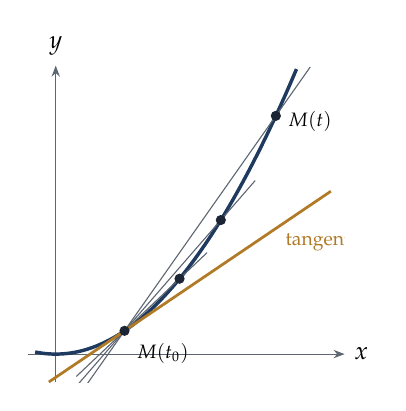
\begin{tikzpicture}
\begin{axis}[courbe,width=5.6cm,height=5.6cm,xmin=-0.2,xmax=2.1,ymin=-0.3,ymax=3.1,xtick=\empty,ytick=\empty,axis equal image=false]
\addplot[arcetude,domain=-0.15:1.75]({x},{x^2});
\addplot[Gris,thin,domain=0.15:1.85,samples=2]{0.25+2.1*(x-0.5)};
\addplot[Gris,thin,domain=0.15:1.45,samples=2]{0.25+1.7*(x-0.5)};
\addplot[Gris,thin,domain=0.15:1.1,samples=2]{0.25+1.4*(x-0.5)};
\addplot[tgte,domain=-0.05:2.0,samples=2]{x-0.25};
\node[pt] at (axis cs:0.5,0.25) {}; \node[font=\scriptsize,anchor=north west] at (axis cs:0.52,0.22) {$M(t_0)$};
\node[pt] at (axis cs:1.6,2.56) {}; \node[pt] at (axis cs:1.2,1.44) {}; \node[pt] at (axis cs:0.9,0.81) {};
\node[font=\scriptsize,anchor=west] at (axis cs:1.62,2.5) {$M(t)$};
\node[font=\scriptsize,Ocre,anchor=west] at (axis cs:1.6,1.2) {tangente};
\end{axis}
\end{tikzpicture}\\
{\scriptsize les cordes pivotent vers la tangente}
\end{columns}
\end{frame}

\begin{frame}{Tangente en un point régulier}
\begin{PROP}[Théorème]
En un point régulier : $T=M(t_0)+\vect f'(t_0)$, d'équation
\[\det\big(\vv{M(t_0)M},f'(t_0)\big)=0\iff y'_0(x-x_0)-x'_0(y-y_0)=0.\]
Horizontale $\iff y'(t_0)=0$ ;\quad verticale $\iff x'(t_0)=0$ \ (point régulier !).
\end{PROP}
\pause
\textbf{Preuve :} Taylor--Young à l'ordre 1, $\vv{M(t_0)M(t_0+h)}=h\big(f'(t_0)+o(1)\big)$, donc
$\ve u_h\to\pm\frac{f'(t_0)}{\|f'(t_0)\|}$ : les deux limites dirigent la même droite.
\end{frame}

\begin{frame}{Exemple : tangente à une ellipse}
\begin{ATOI}
Ellipse $f(\theta)=(2\cos\theta,\sin\theta)$ : tangente en $\theta=\frac\pi4$ ?
\end{ATOI}
\pause
\begin{columns}[c]
\column{0.58\textwidth}
\begin{itemize}
\item $M_0=\big(\sqrt2,\frac{\sqrt2}2\big)$, \ $f'\big(\frac\pi4\big)=\big(-\sqrt2,\frac{\sqrt2}2\big)\neq\ve0$ : régulier.
\pause
\item $y'_0(x-x_0)-x'_0(y-y_0)=0$ :
\[\tfrac{\sqrt2}2(x-\sqrt2)+\sqrt2\big(y-\tfrac{\sqrt2}2\big)=0\]
\[\iff\ \rep{x+2y-2\sqrt2=0}.\]
\end{itemize}
\column{0.38\textwidth}\centering\onslide<1->
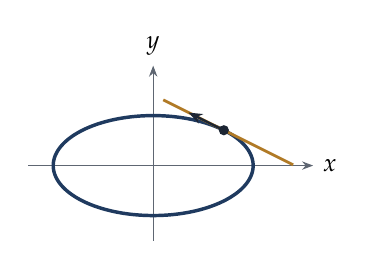
\begin{tikzpicture}
\begin{axis}[courbe,width=5.2cm,xmin=-2.5,xmax=3.2,ymin=-1.5,ymax=2,xtick=\empty,ytick=\empty]
\addplot[arcetude,domain=0:6.2832]({2*cos(x)},{sin(x)});
\uncover<3->{\addplot[tgte,samples=2,domain=0.2:2.8]{(2*sqrt(2)-x)/2};}
\node[pt] at (axis cs:1.414,0.707) {};
\uncover<2->{\draw[->,thick,Ink] (axis cs:1.414,0.707)--(axis cs:0.707,1.06);}
\end{axis}
\end{tikzpicture}
\end{columns}
\end{frame}

% ---------------------------------------------------------------- EXERCICE C1
\begin{frame}{\badgeexo{1}Tangentes horizontales, verticales, en un point}
\begin{ENONCE}[5 min]
Soit $f(t)=\big(t^2,\ t^3-3t\big)$, $t\in\R$.
\begin{enumerate}
\item Déterminer les points où la tangente est horizontale, puis verticale.
\item Donner une équation de la tangente au point de paramètre $t=2$.
\end{enumerate}
\objectif{tangente dirigée par $f'(t)$ en un point régulier.}
\end{ENONCE}
\end{frame}

\begin{frame}{\badgecor{1}Tangentes horizontales, verticales, en un point}
\begin{columns}[T]
\column{0.38\textwidth}
\begin{RAIS}
En un point régulier, la tangente est dirigée par $f'(t)=(x'(t),y'(t))$ : horizontale si $y'=0$, verticale si $x'=0$.
\end{RAIS}
\begin{OUTIL}
Tangente en un point régulier : $\det\big(M-f(t_0),\,f'(t_0)\big)=0$.
\end{OUTIL}
\column{0.59\textwidth}
\etape{1.} $f'(t)=(2t,\ 3t^2-3)$. Horizontale : $t=\pm1$ ($x'\neq0$), points $(1,-2)$ et $(1,2)$.
Verticale : $t=0$ ($y'(0)=-3\neq0$), point $(0,0)$.\\[3pt]
\pause
\etape{2.} $f(2)=(4,2)$, $f'(2)=(4,9)$ :
\[\dt{x-4&4\\y-2&9}=0\iff9x-4y-28=0.\]
\end{columns}
\end{frame}

\begin{frame}{D'où vient la pente $\dfrac{y'}{x'}$ ?}
Si $x'(t_0)\neq0$, $x$ est strictement monotone près de $t_0$ : localement, la courbe est un \textbf{graphe}
\[y(t)=g\big(x(t)\big).\]
\pause
On dérive la composée :\qquad $y'(t)=g'\big(x(t)\big)\,x'(t)$,\qquad donc\qquad
\[\boxed{\ \text{pente}=g'\big(x(t_0)\big)=\frac{y'(t_0)}{x'(t_0)}\ }\]
\pause
\begin{columns}[T]
\column{0.48\textwidth}
\begin{FORM}[Usages]
Parallèle à $\ve w$ : $\det(f',\ve w)=0$.\\
Pente $m$ : $y'=m\,x'$.
\end{FORM}
\column{0.48\textwidth}
\begin{PIEGE}[Pièges]
« $x'=0$ donc verticale » : faux si $y'=0$ aussi.\\
$\frac yx$ = pente de $(OM)$, pas de la tangente.
\end{PIEGE}
\end{columns}
\end{frame}

% =====================================================================
\partie{2.3}{Plan d'étude, symétries, tracé}{Dans quel ordre étudier une courbe pour la tracer sans rien oublier ?}{\rmII}

\begin{frame}{Le plan d'étude en 6 étapes}
\begin{center}
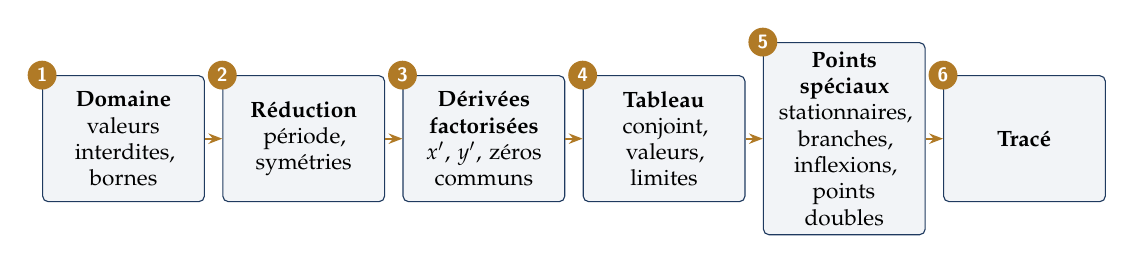
\begin{tikzpicture}[node distance=0.22cm,
  st/.style={rectangle,rounded corners=2pt,draw=Bleu,fill=Fond,text width=1.82cm,minimum height=1.6cm,align=center,font=\footnotesize},
  nb/.style={circle,fill=Ocre,text=white,font=\sffamily\bfseries\scriptsize,inner sep=1.5pt}]
\node[st] (a) {\textbf{Domaine}\\ valeurs interdites, bornes};
\node[st,right=of a] (b) {\textbf{Réduction}\\ période, symétries};
\node[st,right=of b] (c) {\textbf{Dérivées factorisées}\\ $x'$, $y'$, zéros communs};
\node[st,right=of c] (d) {\textbf{Tableau} conjoint, valeurs, limites};
\node[st,right=of d] (e) {\textbf{Points\\ spéciaux}\\ stationnaires, branches, inflexions, points doubles};
\node[st,right=of e] (f) {\textbf{Tracé}};
\foreach \n/\k in {a/1,b/2,c/3,d/4,e/5,f/6}{\node[nb] at (\n.north west) {\k};}
\foreach \x/\y in {a/b,b/c,c/d,d/e,e/f}{\draw[->,Ocre,thick] (\x)--(\y);}
\end{tikzpicture}
\end{center}
\pause
\begin{itemize}
\item Étape 3 : \alert{même dénominateur, facteurs affines} : les signes se lisent directement.
\item Étape 5 : stationnaires (§2.4), branches (§2.5), points doubles (§2.6).
\item Étape 6 : on complète par les symétries \textbf{dans l'ordre inverse} des réductions.
\end{itemize}
\end{frame}

\begin{frame}{Réduire le domaine : les symétries}
\begin{columns}[c]
\column{0.58\textwidth}
\textbf{Principe :} chercher $\varphi$ ($t\mapsto-t$, $\pi-t$, $\frac1t$\dots) telle que $M(\varphi(t))=s\big(M(t)\big)$.
\begin{FORM}[Table des symétries]
\small\renewcommand{\arraystretch}{1.1}
\begin{tabular}{@{}lll@{}}
$f(-t)=(x,-y)$ & axe $(Ox)$ & $t\geq0$\\
$f(-t)=(-x,y)$ & axe $(Oy)$ & $t\geq0$\\
$f(-t)=-f(t)$ & centre $O$ & $t\geq0$\\
$f(\frac1t)=(y,x)$ & axe $y=x$ & $|t|\leq1$\\
$f(\pi-t)=(\pm x,\pm y)$ & selon signes & demi-intervalle\\
$f(t+T)=f(t)$ & période & une période
\end{tabular}
\end{FORM}
\column{0.38\textwidth}\centering\onslide<1->
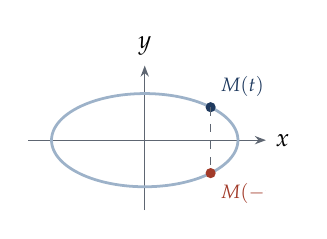
\begin{tikzpicture}
\begin{axis}[courbe,width=4.6cm,xmin=-2.5,xmax=2.6,ymin=-1.5,ymax=1.6,xtick=\empty,ytick=\empty]
\addplot[reste,domain=0:6.2832]({2*cos(x)},{sin(x)});
\node[pt,fill=Bleu] at (axis cs:1.414,0.707) {}; \node[font=\scriptsize,anchor=south west,Bleu] at (axis cs:1.42,0.72) {$M(t)$};
\node[pt,fill=Brique] at (axis cs:1.414,-0.707) {}; \node[font=\scriptsize,anchor=north west,Brique] at (axis cs:1.42,-0.72) {$M(-t)$};
\draw[Gris,dashed] (axis cs:1.414,0.707)--(axis cs:1.414,-0.707);
\end{axis}
\end{tikzpicture}\\
{\scriptsize $x$ paire, $y$ impaire : symétrie d'axe $(Ox)$}
\end{columns}
\end{frame}

% ---------------------------------------------------------------- EXERCICE C2
\begin{frame}{\badgeexo{2}Réduire l'intervalle d'étude}
\begin{ENONCE}[5 min]
Soit $f(t)=\big(\sin2t,\ \sin3t\big)$. Réduire l'intervalle d'étude au maximum, en précisant à chaque étape la transformation
géométrique qui permet de reconstituer la courbe.
\objectif{périodicité, puis $f(-t)$, puis $f(\pi-t)$.}
\end{ENONCE}
\end{frame}

\begin{frame}{\badgecor{2}Réduire l'intervalle d'étude}
\begin{columns}[T]
\column{0.38\textwidth}
\begin{RAIS}
On compare $f(t+T)$, $f(-t)$, $f(a-t)$ à $(\pm x,\pm y)$ : chaque relation divise l'intervalle par $2$ et fournit une symétrie.
\end{RAIS}
\begin{OUTIL}
Réduction par les symétries (§2.3).
\end{OUTIL}
\column{0.59\textwidth}
\etape{1.} $f$ est $2\pi$-périodique : étude sur $[-\pi,\pi]$.\\[3pt]
\etape{2.} $f(-t)=(-x,-y)$ : symétrie de centre $O$ ; étude sur $[0,\pi]$.\\[3pt]
\pause
\etape{3.} $f(\pi-t)=\big(\sin(2\pi-2t),\sin(3\pi-3t)\big)=(-x,\,y)$ : symétrie d'axe $(Oy)$ ; étude sur $\left[0,\frac\pi2\right]$.\\[3pt]
Reconstitution : arc sur $\left[0,\frac\pi2\right]$, symétrique par rapport à $(Oy)$, puis par rapport à $O$.
\end{columns}
\end{frame}

\begin{frame}{Exemple : l'ellipse $f(\theta)=(2\cos\theta,\sin\theta)$}
\begin{columns}[c]
\column{0.55\textwidth}
\begin{enumerate}
\item $2\pi$-périodique.\pause
\item $x$ paire, $y$ impaire : \textbf{axe $(Ox)$}, étude sur $[0,\pi]$.\pause
\item $f(\pi-\theta)=(-x,y)$ : \textbf{axe $(Oy)$}, étude sur $\big[0,\frac\pi2\big]$.\pause
\item Sur $\big[0,\frac\pi2\big]$ : $x\searrow$ de $2$ à $0$, $y\nearrow$ de $0$ à $1$ ; tangente verticale en $(2,0)$
      ($f'(0)=(0,1)$), horizontale en $(0,1)$.\pause
\item Compléter : axe $(Oy)$, puis axe $(Ox)$.
\end{enumerate}
\column{0.4\textwidth}\centering\onslide<1->
\begin{tikzpicture}
\begin{axis}[courbe,width=5.4cm,xmin=-2.5,xmax=2.6,ymin=-1.5,ymax=1.6,xtick={-2,2},ytick={-1,1}]
\only<5->{\addplot[reste,domain=1.5708:3.1416]({2*cos(x)},{sin(x)});}
\only<5->{\addplot[reste,domain=3.1416:6.2832]({2*cos(x)},{sin(x)});}
\only<4->{\addplot[arcetude,domain=0:1.5708]({2*cos(x)},{sin(x)});
\addplot[tgte,samples=2,domain=-0.4:0.4]({2},{x});\addplot[tgte,samples=2,domain=-0.6:0.6]({x},{1});}
\end{axis}
\end{tikzpicture}\\
{\scriptsize arc étudié (foncé), puis complété par symétries}
\end{columns}
\end{frame}

\begin{frame}{Du tableau au tracé}
\begin{columns}[c]
\column{0.4\textwidth}\centering\onslide<1->
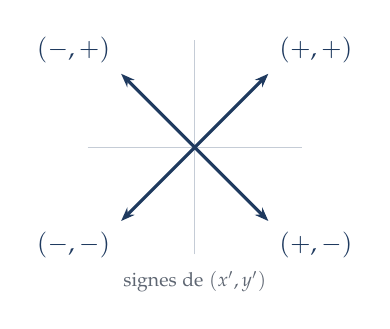
\begin{tikzpicture}[scale=0.85]
\draw[Filet] (-1.6,0)--(1.6,0) (0,-1.6)--(0,1.6);
\draw[->,Bleu,very thick] (0,0)--(1.1,1.1) node[above right,font=\small]{$(+,+)$};
\draw[->,Bleu,very thick] (0,0)--(1.1,-1.1) node[below right,font=\small]{$(+,-)$};
\draw[->,Bleu,very thick] (0,0)--(-1.1,1.1) node[above left,font=\small]{$(-,+)$};
\draw[->,Bleu,very thick] (0,0)--(-1.1,-1.1) node[below left,font=\small]{$(-,-)$};
\node[font=\scriptsize,Gris] at (0,-2) {signes de $(x',y')$};
\end{tikzpicture}
\column{0.56\textwidth}
\begin{METH}{Tracer}
\begin{enumerate}
\item Asymptotes en pointillés ; points nommés avec un segment de tangente.
\item Arcs selon le tableau : direction donnée par les signes de $(x',y')$.
\item Positions (asymptotes, tangentes) ; symétries ; flèches de sens.
\end{enumerate}
\end{METH}
\end{columns}
\pause
\begin{ASTU}[Astuces]
Point sur un axe de symétrie : tangente $\perp$ à l'axe, sauf point stationnaire ou double.
Symétrie supposée : vérifier la compatibilité ($f$ impaire $\Rightarrow f(0)=O$).
\end{ASTU}
\end{frame}

% =====================================================================
\partie{2.4}{Points stationnaires, étude locale, inflexions}{Que se passe-t-il quand la vitesse s'annule ? Quand la courbe traverse-t-elle sa tangente ?}{\rmII}

\begin{frame}{Les quatre allures locales}
\begin{center}
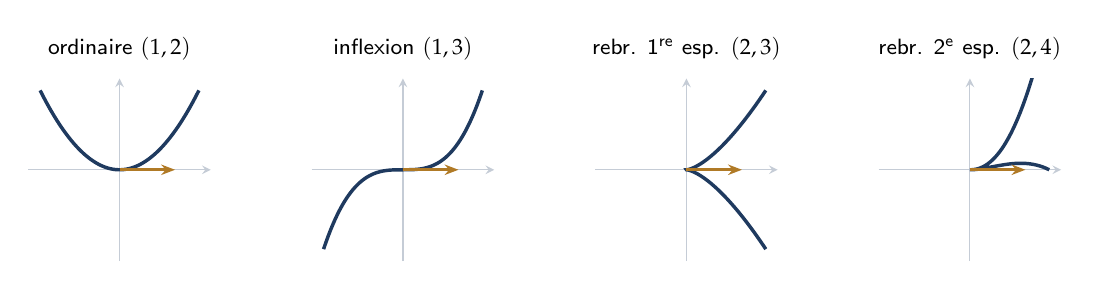
\begin{tikzpicture}
\begin{axis}[mini,title={ordinaire $(1,2)$}]\addplot[arcetude,domain=-1:1]({x},{x^2});\draw[tgte,->](axis cs:0,0)--(axis cs:0.7,0);\end{axis}
\begin{axis}[mini,xshift=3.6cm,title={inflexion $(1,3)$}]\addplot[arcetude,domain=-1:1]({x},{x^3});\draw[tgte,->](axis cs:0,0)--(axis cs:0.7,0);\end{axis}
\begin{axis}[mini,xshift=7.2cm,title={rebr. 1\textsuperscript{re} esp. $(2,3)$}]\addplot[arcetude,domain=-1:1]({x^2},{x^3});\draw[tgte,->](axis cs:0,0)--(axis cs:0.7,0);\end{axis}
\begin{axis}[mini,xshift=10.8cm,title={rebr. 2\textsuperscript{e} esp. $(2,4)$}]\addplot[arcetude,domain=-1:1]({x^2},{x^4+x^5});\draw[tgte,->](axis cs:0,0)--(axis cs:0.7,0);\end{axis}
\end{tikzpicture}
\end{center}
\pause
\begin{DEF}
\textbf{Ordinaire} : la courbe reste du même côté de sa tangente. \textbf{Inflexion} : elle la traverse.
\textbf{Rebroussement} : elle s'arrête et repart en arrière, en traversant sa tangente (1\textsuperscript{re} espèce) ou non
(2\textsuperscript{e}). \textbf{Anguleux} : demi-tangentes non colinéaires ($(t,|t|)$).
\end{DEF}
\pause
Modèle $(t^p,t^q)$ en $O$ : la corde $\frac{(t^p,t^q)}{t^p}=(1,t^{q-p})\to(1,0)$ ; les \textbf{parités} de $p,q$ décident.
\end{frame}

\begin{frame}{Le théorème $(p,q)$}
\begin{PROP}[Théorème $(p,q)$]
$p=\min\{k\geq1:f^{(k)}(t_0)\neq\ve0\}$, \ $q=\min\{k>p:(f^{(p)},f^{(k)})\text{ libre}\}$. Tangente dirigée par $f^{(p)}(t_0)$.
\begin{center}
\renewcommand{\arraystretch}{1.2}
\begin{tabular}{c|cc}
 & $q$ pair & $q$ impair\\\hline
$p$ impair & ordinaire & inflexion\\
$p$ pair & rebr. 2\textsuperscript{e} esp. & rebr. 1\textsuperscript{re} esp.
\end{tabular}
\end{center}
\end{PROP}
\pause
\textbf{Pourquoi :} dans le repère $\big(M_0,f^{(p)}(t_0),f^{(q)}(t_0)\big)$, \ $X\sim\frac{h^p}{p!}$, $Y\sim\frac{h^q}{q!}$.
\begin{itemize}
\item $p$ impair : $X$ change de signe, la courbe \emph{passe} ; $p$ pair : elle \emph{rebrousse}.
\item $q$ impair : $Y$ change de signe, la courbe \emph{traverse} sa tangente.
\end{itemize}
\end{frame}

% ---------------------------------------------------------------- EXERCICE C3
\begin{frame}{\badgeexo{3}Trois points stationnaires}
\begin{ENONCE}[6 min]
Pour chaque courbe, déterminer $p$ et $q$ au point de paramètre $0$, puis l'allure locale.
\[\text{(a)}\ \big(t^2,\ t^3\big)\qquad\text{(b)}\ \big(t^3,\ t^5\big)\qquad\text{(c)}\ \big(t^2,\ t^4+t^5\big)\]
\objectif{appliquer le théorème $(p,q)$.}
\end{ENONCE}
\pause
\begin{INDICE}
$p$ : premier ordre de dérivée non nulle ; $q$ : premier ordre où la dérivée n'est plus colinéaire à $f^{(p)}(0)$.
\end{INDICE}
\end{frame}

\begin{frame}{\badgecor{3}Trois points stationnaires}
\begin{columns}[T]
\column{0.38\textwidth}
\begin{RAIS}
Les coordonnées sont des polynômes : les dérivées en $0$ se lisent sur les coefficients. Parités de $p$ et $q$ $\Rightarrow$ allure.
\end{RAIS}
\begin{OUTIL}
Théorème $(p,q)$ (§2.4).
\end{OUTIL}
\column{0.59\textwidth}
\etape{(a)} $f''(0)=(2,0)$, $f'''(0)=(0,6)$ : $p=2$, $q=3$ : \textbf{rebroussement de première espèce}.\\[3pt]
\pause
\etape{(b)} $f'''(0)=(6,0)$, $f^{(5)}(0)=(0,120)$ : $p=3$, $q=5$, impairs : \textbf{inflexion}.\\[3pt]
\pause
\etape{(c)} $f''(0)=(2,0)$, $f'''(0)=(0,0)$, $f^{(4)}(0)=(0,24)$ : $p=2$, $q=4$ : \textbf{rebroussement de seconde espèce}.
\end{columns}
\end{frame}

\begin{frame}{Méthode : étudier un point par développement limité}
\begin{METH}{Point stationnaire par DL}
\begin{enumerate}
\item $t=t_0+h$ ; DL de $x$ et $y$.
\item $f(t_0+h)=f(t_0)+h^p\ve a+\dots+h^q\ve b+o(h^q)$ : s'arrêter au \textbf{premier} $\ve b$ avec $\det(\ve a,\ve b)\neq0$.
\item Tangente : $M_0+\vect\ve a$, équation $\det(\vv{M_0M},\ve a)=0$ \ (\alert{pas} $f'(t_0)=\ve0$).
\item Position : du côté de $\ve b$ quand $h^q>0$.
\end{enumerate}
\end{METH}
\pause
\begin{PIEGE}[Pièges]
Terme intermédiaire colinéaire au premier : il ne compte pas. Terme nul : aller plus loin (TD 7).\\
Stationnaire $\not\Rightarrow$ rebroussement : $(t^3,t^5)$ inflexion, $(t^3,t^4)$ ordinaire.
\end{PIEGE}
\end{frame}

\begin{frame}{Exemple : $f(t)=\big(t-2\sqrt{1+t},\ t\ln(1-t)\big)$ en $0$}
\pause
\textbf{DL :} $\sqrt{1+t}=1+\frac t2-\frac{t^2}8+\frac{t^3}{16}+o(t^3)$, \ $\ln(1-t)=-t-\frac{t^2}2+o(t^2)$.
\pause
\[x(t)=-2+\frac{t^2}4-\frac{t^3}8+o(t^3),\qquad y(t)=-t^2-\frac{t^3}2+o(t^3).\]
\pause
\[f(t)=(-2,0)+\frac{t^2}4\underbrace{(1,-4)}_{\ve a}+\frac{t^3}8\underbrace{(-1,-4)}_{\ve b}+o(t^3),\qquad
\det(\ve a,\ve b)=-4-4=-8\neq0.\]
\pause
\begin{columns}[c]
\column{0.62\textwidth}
\begin{RETENIR}
$p=2$, $q=3$ : \textbf{rebroussement de 1\textsuperscript{re} espèce} en $(-2,0)$, tangente dirigée par $(1,-4)$.
\end{RETENIR}
\column{0.34\textwidth}\centering
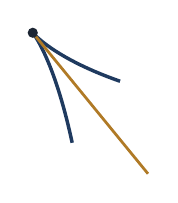
\begin{tikzpicture}
\begin{axis}[width=4.4cm,height=4.4cm,axis lines=none,xmin=-2.12,xmax=-1.6,ymin=-1.4,ymax=0.3,samples=120,smooth]
\addplot[arcetude,domain=-0.7:0.7]({x-2*sqrt(1+x)},{x*ln(1-x)});
\addplot[tgte,samples=2,domain=0:0.27]({-2+x},{-4*x});
\node[pt] at (axis cs:-2,0) {};
\end{axis}
\end{tikzpicture}
\end{columns}
\end{frame}

\begin{frame}{Inflexion : d'où vient $\det(f',f'')$ ?}
Pour un graphe $y=g(x)$ : la courbe est au-dessus de ses tangentes si $g''>0$, au-dessous si $g''<0$.
\pause
Près d'un point régulier où $x'\neq0$ : $y(t)=g\big(x(t)\big)$. On dérive deux fois :
\[y'=g'(x)\,x',\qquad y''=g''(x)\,x'^2+g'(x)\,x''.\]
\pause
On élimine $g'(x)=\frac{y'}{x'}$ :
\[\boxed{\ g''\big(x(t)\big)=\frac{x'y''-y'x''}{x'^3}=\frac{\det(f',f'')}{x'^3}\ }\]
\pause
\begin{columns}[c]
\column{0.55\textwidth}
$x'^3$ garde un signe près de $t_0$ : \textbf{le signe de $\det(f',f'')$ dit de quel côté de ses tangentes est la courbe.}
\column{0.4\textwidth}\centering\onslide<1->
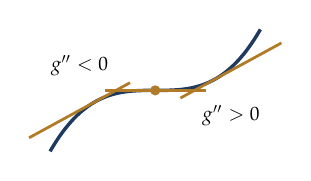
\begin{tikzpicture}
\begin{axis}[width=5cm,height=3.3cm,axis lines=none,xmin=-1.6,xmax=1.6,ymin=-1.3,ymax=1.3,samples=100]
\addplot[arcetude,domain=-1.25:1.25]{0.6*x^3};
\addplot[tgte,domain=-1.5:-0.3,samples=2]{0.6*(-0.343)+1.8*0.49*(x+0.7)};
\addplot[tgte,domain=0.3:1.5,samples=2]{0.6*0.343+1.8*0.49*(x-0.7)};
\addplot[tgte,domain=-0.6:0.6,samples=2]{0};
\node[font=\scriptsize,anchor=south] at (axis cs:-0.9,0.1) {$g''<0$};
\node[font=\scriptsize,anchor=north] at (axis cs:0.9,-0.1) {$g''>0$};
\node[pt,fill=Ocre] at (axis cs:0,0) {};
\end{axis}
\end{tikzpicture}
\end{columns}
\end{frame}

\begin{frame}{Inflexion : les conséquences}
\begin{FORM}[Inflexion et $\det(f',f'')$]
\begin{itemize}
\item Inflexion (point régulier) $\iff\det(f',f'')$ \textbf{change de signe}. Nécessaire : $\det=0$.
\item Birégulier ($\det\neq0$) : point ordinaire, courbe du côté de $f''$.
\item Pente : $p'=\dfrac{\det(f',f'')}{x'^2}$ $\Rightarrow$ pente \textbf{extrémale} à l'inflexion (racine double de $p(t)=m$).
\item Si $x'=0$ : $x=h(y)$, $h''=-\dfrac{\det(f',f'')}{y'^3}$.
\end{itemize}
\end{FORM}
\end{frame}

\begin{frame}{Piège : colinéarité, pas annulation}
\begin{PIEGE}
C'est la \textbf{colinéarité} $f''\parallel f'$ qui compte, pas $f''=\ve0$.
\end{PIEGE}
\begin{columns}[T]
\column{0.48\textwidth}\centering
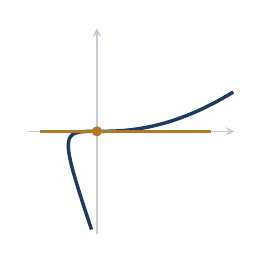
\begin{tikzpicture}
\begin{axis}[mini,width=4.2cm,height=4.2cm,xmin=-0.6,xmax=1.2,ymin=-0.9,ymax=0.9]
\addplot[arcetude,domain=-0.95:0.7]({x+x^2},{x^3});\draw[tgte](axis cs:-0.5,0)--(axis cs:1,0);\node[pt,fill=Ocre] at (axis cs:0,0){};
\end{axis}
\end{tikzpicture}\\
$(t+t^2,t^3)$ : $f''(0)=(2,0)\neq\ve0$,\\ $\det=6t(t+1)$ \textbf{change de signe} :\\ \rep{inflexion}.
\column{0.48\textwidth}\centering
\pause
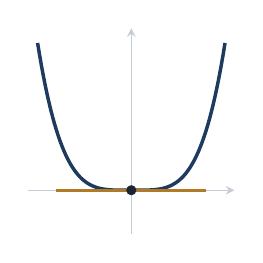
\begin{tikzpicture}
\begin{axis}[mini,width=4.2cm,height=4.2cm,xmin=-1.1,xmax=1.1,ymin=-0.3,ymax=1.1]
\addplot[arcetude,domain=-1:1]({x},{x^4});\draw[tgte](axis cs:-0.8,0)--(axis cs:0.8,0);\node[pt] at (axis cs:0,0){};
\end{axis}
\end{tikzpicture}\\
$(t,t^4)$ : $f''(0)=\ve0$,\\ $\det=12t^2\geq0$ : \rep{pas d'inflexion}.
\end{columns}
\end{frame}

\begin{frame}{Méthode : chercher les inflexions}
\begin{METH}{Chercher les inflexions}
\begin{enumerate}
\item \textbf{Factoriser la vitesse} : $f'=\lambda\ve g$, $\lambda$ scalaire $\neq0$ $\Rightarrow\det(f',f'')=\lambda^2\det(\ve g,\ve g')$.
\item Résoudre $\det(\ve g,\ve g')=0$ aux points réguliers ; trigonométrique : linéariser.
\item Confirmer : changement de signe, ou $\det(f',f''')\neq0$ ($q=3$). Stationnaires : par DL ($p,q$ impairs).
\end{enumerate}
\end{METH}
\pause
\textbf{Pourquoi factoriser ?} \ $f''=\lambda'\ve g+\lambda\ve g'$, donc
\[\det(f',f'')=\det(\lambda\ve g,\lambda'\ve g+\lambda\ve g')=\lambda\lambda'\underbrace{\det(\ve g,\ve g)}_{0}+\lambda^2\det(\ve g,\ve g').\]
\pause
{\small Trigonométrique : factoriser par l'angle moitié, $\cos t-\cos2t=2\sin\frac t2\sin\frac{3t}2$ (§2.1).}
\end{frame}

% =====================================================================
\partie{2.5}{Branches infinies, positions}{Quand le point part à l'infini, la courbe s'approche-t-elle d'une droite ?}{\rmII}

\begin{frame}{Asymptote : définition et critère}
\begin{DEF}
$\|\vv{OM(t)}\|\to\infty$ quand $t\to t_0$ : $\mathcal D$ est \textbf{asymptote} si $d\big(M(t),\mathcal D\big)\to0$.
\end{DEF}
\begin{FORM}[Distance point--droite]
\[d\big(M_0,\ ax+by+c=0\big)=\frac{|ax_0+by_0+c|}{\sqrt{a^2+b^2}}.\]
\end{FORM}
\pause
Pour $\mathcal D:y=\alpha x+\beta$ :\quad $d\to0\iff y-\alpha x\to\beta$.\quad En divisant par $x$ : $\frac yx\to\alpha$.
\pause
\begin{RETENIR}
D'abord $\lim\frac yx=\alpha$ (la \emph{direction}), \textbf{puis} $\lim(y-\alpha x)=\beta$ (la \emph{position} de la droite).
La première limite seule ne prouve rien.
\end{RETENIR}
\end{frame}

\begin{frame}{Classer une branche infinie}
\begin{center}
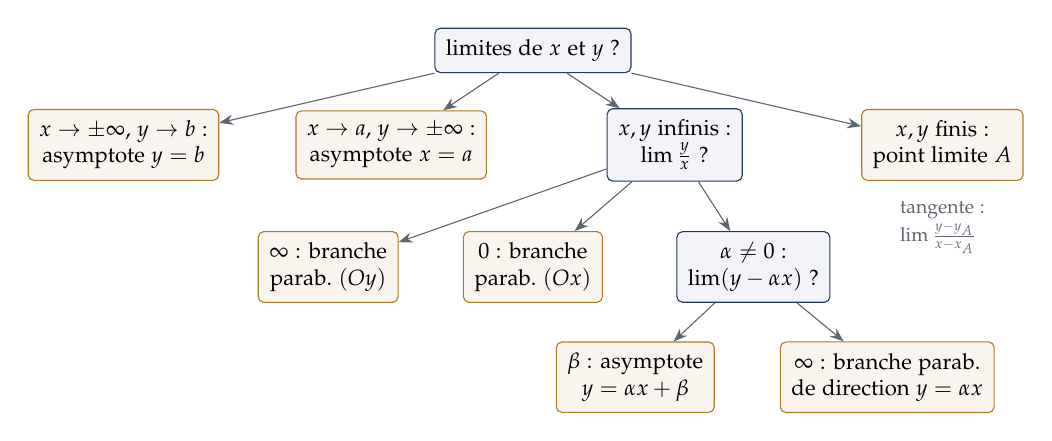
\begin{tikzpicture}[font=\footnotesize,
  q/.style={rectangle,rounded corners=2pt,draw=Bleu,fill=Fond,align=center,inner sep=4pt},
  r/.style={rectangle,rounded corners=2pt,draw=Ocre,fill=Ocre!8,align=center,inner sep=4pt},
  l/.style={font=\scriptsize,Gris}, ->]
\node[q] (a) at (0,0) {limites de $x$ et $y$ ?};
\node[r] (h) at (-5.2,-1.2) {$x\to\pm\infty$, $y\to b$ :\\ asymptote $y=b$};
\node[r] (v) at (-1.8,-1.2) {$x\to a$, $y\to\pm\infty$ :\\ asymptote $x=a$};
\node[q] (b) at (1.8,-1.2) {$x,y$ infinis :\\ $\lim\frac yx$ ?};
\node[r] (pl) at (5.2,-1.2) {$x,y$ finis :\\ point limite $A$};
\draw[Gris] (a)--(h); \draw[Gris] (a)--(v); \draw[Gris] (a)--(b); \draw[Gris] (a)--(pl);
\node[r] (oy) at (-2.6,-2.75) {$\infty$ : branche\\ parab.\ $(Oy)$};
\node[r] (ox) at (0,-2.75) {$0$ : branche\\ parab.\ $(Ox)$};
\node[q] (c) at (2.8,-2.75) {$\alpha\neq0$ :\\ $\lim(y-\alpha x)$ ?};
\draw[Gris] (b)--(oy); \draw[Gris] (b)--(ox); \draw[Gris] (b)--(c);
\node[r] (as) at (1.3,-4.15) {$\beta$ : asymptote\\ $y=\alpha x+\beta$};
\node[r] (bp) at (4.5,-4.15) {$\infty$ : branche parab.\\ de direction $y=\alpha x$};
\draw[Gris] (c)--(as); \draw[Gris] (c)--(bp);
\node[l,align=left,anchor=north] at (5.2,-1.8) {tangente :\\ $\lim\frac{y-y_A}{x-x_A}$};
\end{tikzpicture}
\end{center}
\vspace{-0.15cm}
{\small Pour \textbf{chaque} borne et valeur interdite. Position : signe de $y-\alpha x-\beta$ (développement asymptotique).}
\end{frame}

% ---------------------------------------------------------------- EXERCICE C4
\begin{frame}{\badgeexo{4}Une branche infinie}
\begin{ENONCE}[6 min]
Soit $f(t)=\left(\dfrac t{t-1},\ \dfrac{t^2}{t-1}\right)$. Étudier la branche infinie quand $t\to1$ : direction asymptotique,
asymptote éventuelle, position de la courbe.
\objectif{$\frac yx$, puis $y-\alpha x$, puis le signe de l'écart.}
\end{ENONCE}
\end{frame}

\begin{frame}{\badgecor{4}Une branche infinie}
\begin{columns}[T]
\column{0.38\textwidth}
\begin{RAIS}
$x$ et $y$ tendent vers l'infini : on cherche la pente $\alpha=\lim\frac yx$, puis $\lim(y-\alpha x)$.
\end{RAIS}
\begin{OUTIL}
Classification des branches infinies (§2.5).
\end{OUTIL}
\column{0.59\textwidth}
\etape{1.} $\frac yx=t\to1$ : direction asymptotique de pente $1$.\\[3pt]
\pause
\etape{2.} $y-x=\frac{t^2-t}{t-1}=t\to1$ : \textbf{asymptote} $y=x+1$.\\[3pt]
\pause
\etape{3.} $y-(x+1)=t-1$ : la courbe est au-dessus de l'asymptote pour $t>1$, en dessous pour $t<1$.
\end{columns}
\end{frame}

\begin{frame}{Exemple : une asymptote oblique \ajout}
\[x(t)=t+\frac1{t-1},\qquad y(t)=t^2+\frac2{t-1},\qquad t\neq1.\]
\begin{columns}[c]
\column{0.58\textwidth}
\pause
\textbf{$t\to1$ :} $x,y\to\infty$ ; $\dfrac yx=\dfrac{t^2(t-1)+2}{t(t-1)+1}\to2$.
\pause\par\smallskip
$y-2x=t^2-2t\to-1$ : \textbf{asymptote} $y=2x-1$.
\pause\par\smallskip
Position : $y-2x+1=t^2-2t+1=(t-1)^2>0$ : \rep{courbe au-dessus}, des deux côtés.
\pause\par\smallskip
\textbf{$t\to\pm\infty$ :} $x\sim t$, $y\sim t^2$, $\frac yx\to\pm\infty$ : branche parabolique de direction $(Oy)$.
\column{0.4\textwidth}\centering\onslide<1->
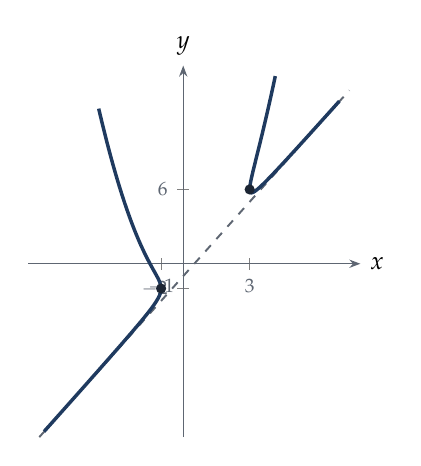
\begin{tikzpicture}
\begin{axis}[courbe,width=5.8cm,height=6.3cm,axis equal image=false,xmin=-7,xmax=8,ymin=-14,ymax=16,xtick={-1,3},ytick={-2,6},
  restrict y to domain=-14:16,restrict x to domain=-7:8]
\addplot[asy,domain=-6.5:7.5,samples=2]{2*x-1};
\only<2->{\addplot[arcetude,domain=-3.6:0.86,samples=300]({x+1/(x-1)},{x^2+2/(x-1)});
\addplot[arcetude,domain=1.17:3.8,samples=300]({x+1/(x-1)},{x^2+2/(x-1)});
\node[pt] at (axis cs:-1,-2) {}; \node[pt] at (axis cs:3,6) {};}
\end{axis}
\end{tikzpicture}
\end{columns}
\end{frame}

\begin{frame}{Position globale par rapport à une droite}
\begin{METH}{Position globale}
$\varphi(t)=ax(t)+by(t)+c$ :
\begin{itemize}
\item zéros de $\varphi$ = points d'intersection avec $ax+by+c=0$ ;
\item signe de $\varphi$ = côté ($b<0$ : $\varphi>0$ signifie au-dessous) ;
\item tangente en $M(t_0)$ : $t_0$ racine \textbf{double} de $\varphi$, donc $(t-t_0)$ facteur de $\varphi'$.
\end{itemize}
\end{METH}
\pause
Dans l'exemple : $\varphi(t)=y-2x+1=(t-1)^2$ ne s'annule jamais pour $t\neq1$ : la courbe ne coupe pas son asymptote.
\pause
\begin{PIEGE}[Pièges]
Oublier une borne du domaine. Factoriser le dénominateur ($1+t^3=(1+t)(1-t+t^2)$) avant de calculer $y-\alpha x$.
Un carré au numérateur de $y-\alpha x-\beta$ : même côté des deux côtés.
\end{PIEGE}
\end{frame}

\begin{frame}{Point limite ; pour aller plus loin \HP}
\textbf{Limites finies :} $M(t)\to A$. On place $A$ (cercle creux s'il n'est pas atteint) ; la tangente est la limite de la
corde : $\lim\frac{y-y_A}{x-x_A}$. Si $A=O$ : c'est $\lim\frac yx$ (la corde issue de $O$ tend vers la tangente).
\pause
\begin{HPBOX}
\textbf{Courbe asymptote} $\Gamma$ : exhiber $P_t\in\Gamma$ avec $M(t)P_t\to0$. Même abscisse : $y-g(x)\to0$ (parabole :
$y-\frac{x^2}2\to0$). Pour une exponentielle, à même ordonnée, $x-\ln(y-c)\to0$ est vrai pour \emph{toute} constante $c$ ;
seule la distance verticale en privilégie une.\\[2pt]
\textbf{Polaires} : $x=r\cos\theta$, $y=r\sin\theta$, partir de $x^2+y^2=r^2$. Cardioïde $r=1-\cos\theta$ ;
lemniscate $(x^2+y^2)^2=xy$, $r^2=\frac12\sin2\theta$.
\end{HPBOX}
\end{frame}

% =====================================================================
\partie{2.6}{Intersections, points doubles}{Comment trouver les points où la courbe se recoupe, ou recoupe une droite ?}{\rmII}

\begin{frame}{Deux méthodes}
\begin{METH}{Intersection courbe/droite}
Substituer $x(t)$, $y(t)$ dans l'équation de la droite. Trigonométrique : tout en $X=\cos t$, élever au carré
($\sin^2t=1-X^2$), factoriser ; \textbf{vérifier les signes} à la fin. Tangence : racine double.
\end{METH}
\pause
\begin{METH}{Points doubles}
Résoudre $f(t)=f(s)$, $t\neq s$ ; une symétrie aide (point de l'axe $(Oy)$ : $x(t)=0$).\\
Sans formule (tableau) : écrire deux arcs comme graphes et appliquer le TVI à $h_1-h_2$ (TD 1).\\
Tangentes au point double : une par paramètre.
\end{METH}
\pause
\textbf{Synthèse :} on applique tout le chapitre à une courbe de Lissajous.
\end{frame}

\begin{frame}{Synthèse : $f(t)=(\cos3t,\ 2\sin t)$ --- réduction}
\begin{columns}[c]
\column{0.56\textwidth}
\begin{itemize}
\item $2\pi$-périodique ; $f(-t)=(x,-y)$ : axe $(Ox)$ ;\\ $f(\pi-t)=(-x,y)$ : axe $(Oy)$.\\
      Étude sur $\big[0,\frac\pi2\big]$.
\pause
\item $x'=-3\sin3t$ (nul en $0$, $\frac\pi3$), $y'=2\cos t>0$ sauf en $\frac\pi2$ : courbe \textbf{régulière}.
\pause
\item $x$ : $1\searrow-1$ ($t=\frac\pi3$) $\nearrow0$ ; \ $y$ : $0\nearrow2$.
\item Tangentes verticales en $(1,0)$ et $(-1,\sqrt3)$, horizontale en $(0,2)$.
\end{itemize}
\column{0.4\textwidth}\centering\onslide<1->
\begin{tikzpicture}
\begin{axis}[courbe,width=4.6cm,height=7cm,xmin=-1.35,xmax=1.35,ymin=-2.3,ymax=2.3,xtick={-1,1},ytick={-2,2}]
\only<3->{\addplot[reste,domain=0:6.2832,samples=400]({cos(3*x)},{2*sin(x)});}
\only<2->{\addplot[arcetude,domain=0:1.5708,samples=200]({cos(3*x)},{2*sin(x)});}
\end{axis}
\end{tikzpicture}
\end{columns}
\end{frame}

\begin{frame}{Synthèse --- point double et tangentes}
\begin{columns}[c]
\column{0.56\textwidth}
\begin{ATOI}
$x(t)=0$ et $y(t)=1$ : pour quels $t\in[0,\pi]$ ?
\end{ATOI}
\pause
$\sin t=\frac12$ : $t=\frac\pi6$ ou $\frac{5\pi}6$, et $\cos3t=0$ dans les deux cas : \rep{point double $J=(0,1)$}.
\pause
\[f'\big(\tfrac\pi6\big)=(-3,\sqrt3),\qquad f'\big(\tfrac{5\pi}6\big)=(-3,-\sqrt3).\]
\pause
\[T_1:\ y=-\frac x{\sqrt3}+1,\qquad T_2:\ y=\frac x{\sqrt3}+1.\]
\column{0.4\textwidth}\centering\onslide<1->
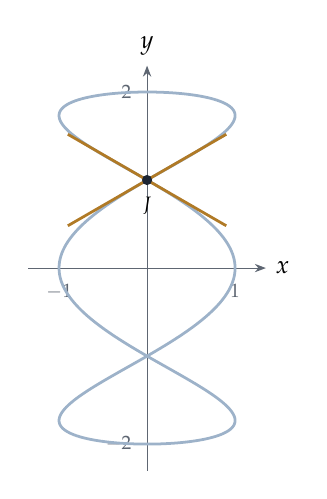
\begin{tikzpicture}
\begin{axis}[courbe,width=4.6cm,height=7cm,xmin=-1.35,xmax=1.35,ymin=-2.3,ymax=2.3,xtick={-1,1},ytick={-2,2}]
\addplot[reste,domain=0:6.2832,samples=400]({cos(3*x)},{2*sin(x)});
\only<4->{\addplot[tgte,domain=-0.9:0.9,samples=2]{-x/sqrt(3)+1};
\addplot[tgte,domain=-0.9:0.9,samples=2]{x/sqrt(3)+1};}
\node[pt] at (axis cs:0,1) {}; \node[font=\scriptsize,anchor=north] at (axis cs:0,0.92) {$J$};
\end{axis}
\end{tikzpicture}
\end{columns}
\end{frame}

\begin{frame}{Synthèse --- où $T_2$ recoupe-t-elle la courbe ?}
$M(t)\in T_2\iff2\sin t=\frac{\cos3t}{\sqrt3}+1$. \ On pose $X=\cos t$, $\cos3t=4X^3-3X$ :\ \ $2\sqrt3\sin t=4X^3-3X+\sqrt3$.
\pause
\par\smallskip
On élève au carré ($\sin^2t=1-X^2$) :
\begin{align*}P(X)&=(4X^3-3X+\sqrt3)^2-12(1-X^2)\\&=16\Big(X-\tfrac{\sqrt3}2\Big)\Big(X+\tfrac{\sqrt3}2\Big)^2\Big(X^3-\tfrac{\sqrt3}2X^2+\tfrac{\sqrt3}2\Big).\end{align*}
\pause
\begin{itemize}
\item $X=-\frac{\sqrt3}2$, \textbf{racine double} : la tangence ($t=\frac{5\pi}6$) ;\ \ $X=\frac{\sqrt3}2$ : l'autre branche par $J$.
\item Dernier facteur : une racine réelle $X_0\approx-0{,}735$.
\end{itemize}
\pause
\begin{PIEGE}[Vérifier le signe (élévation au carré)]
$\sin t=\frac{4X_0^3-3X_0+\sqrt3}{2\sqrt3}\approx0{,}68>0$ : convient. \ Un seul autre point : $K\approx(0{,}62\,;\,1{,}36)$.
\end{PIEGE}
\end{frame}

\begin{frame}{Synthèse --- inflexions}
\begin{columns}[c]
\column{0.58\textwidth}
\[\det(f',f'')=\dt{-3\sin3t&-9\cos3t\\2\cos t&-2\sin t}\]\[=6(\sin3t\sin t+3\cos3t\cos t).\]
\pause
\textbf{Linéariser} (plus court que $\tan$) :
\[\det=12\cos2t+6\cos4t=6(2c^2+2c-1)\]
avec $c=\cos2t$ (car $\cos4t=2c^2-1$).
\pause
Nul pour $c=\frac{\sqrt3-1}2$ : sur $\big[0,\frac\pi2\big]$, seul $\alpha\approx0{,}598$, où $\det$ \textbf{change de signe}.
\pause
\begin{RETENIR}
$M(\alpha)\approx(-0{,}22\,;\,1{,}13)$ est une inflexion ; par symétrie, \textbf{quatre} inflexions.
\end{RETENIR}
\column{0.38\textwidth}\centering\onslide<1->
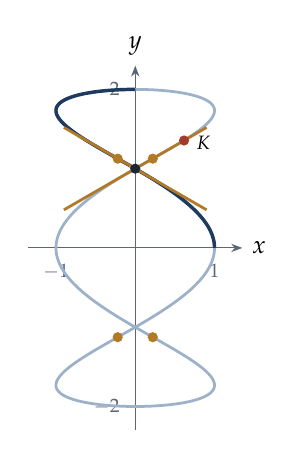
\begin{tikzpicture}
\begin{axis}[courbe,width=4.3cm,height=6.4cm,xmin=-1.35,xmax=1.35,ymin=-2.3,ymax=2.3,xtick={-1,1},ytick={-2,2}]
\addplot[reste,domain=0:6.2832,samples=400]({cos(3*x)},{2*sin(x)});
\addplot[arcetude,domain=0:1.5708,samples=200]({cos(3*x)},{2*sin(x)});
\addplot[tgte,domain=-0.9:0.9,samples=2]{-x/sqrt(3)+1};
\addplot[tgte,domain=-0.9:0.9,samples=2]{x/sqrt(3)+1};
\node[pt] at (axis cs:0,1) {};
\node[pt,fill=Brique] at (axis cs:0.6154,1.3553) {}; \node[font=\scriptsize,anchor=west] at (axis cs:0.65,1.33) {$K$};
\only<4->{\node[pt,fill=Ocre] at (axis cs:-0.2214,1.126) {}; \node[pt,fill=Ocre] at (axis cs:0.2214,1.126) {};
\node[pt,fill=Ocre] at (axis cs:-0.2214,-1.126) {}; \node[pt,fill=Ocre] at (axis cs:0.2214,-1.126) {};}
\end{axis}
\end{tikzpicture}
\end{columns}
\end{frame}

% =====================================================================
\partie{2.7}{Check-list et résultats des TD}{Avant de rendre une étude de courbe : ai-je tout vérifié ?}{\rmII}

\begin{frame}{La check-list d'une étude}
\begin{columns}[T]
\column{0.5\textwidth}
\begin{enumerate}
\item Domaine, valeurs interdites ; symétries \textbf{vérifiées}.
\item Dérivées \textbf{factorisées} ; zéros communs.
\item Tangentes : régularité vérifiée.
\item DL jusqu'au premier vecteur non colinéaire.
\end{enumerate}
\column{0.48\textwidth}
\begin{enumerate}\setcounter{enumi}{4}
\item \textbf{Toutes} les branches ; $\lim(y-\alpha x)$ ; position.
\item Position globale : $\varphi$ ; inflexions : $\lambda\ve g$.
\item Élévation au carré : signes.
\item Tracé fidèle (positions, tangentes, symétries).
\end{enumerate}
\end{columns}
\pause
\begin{RETENIR}
\begin{itemize}
\item Tangente : $M(t_0)+\vect f'(t_0)$ si régulier ; sinon le premier vecteur non nul du DL.
\item Nature locale : parités de $(p,q)$. \quad Concavité : signe de $\det(f',f'')$.
\item Asymptote : $\lim\frac yx$, \textbf{puis} $\lim(y-\alpha x)$, puis position.
\end{itemize}
\end{RETENIR}
\pause
\textbf{Au travail :} TD 1 à 10 de courbes, avec la fiche (§2.7 : résultats des TD pour se corriger).
\end{frame}

\begin{frame}[plain]
\begin{tikzpicture}[remember picture,overlay]
  \fill[Bleu] (current page.north west) rectangle (current page.south east);
  \node[anchor=north west,text=white,font=\sffamily\bfseries\LARGE] at ([xshift=1cm,yshift=-1.4cm]current page.north west) {Après la séance};
  \node[anchor=north west,text width=13.5cm,text=white,font=\normalsize] at ([xshift=1cm,yshift=-2.6cm]current page.north west)
   {\color{white}\setbeamercolor{normal text}{fg=white}\usebeamercolor[fg]{normal text}\begin{itemize}\itemsep6pt
    \item[\textcolor{Ocre}{\rule{0.4em}{0.4em}}] Relire le \textbf{livret} du chapitre ; la \textbf{fiche} reprend chaque partie sous le même numéro (§2.1 à §2.7).
    \item[\textcolor{Ocre}{\rule{0.4em}{0.4em}}] Réviser : refaire les exemples et les exercices des diapositives sans regarder la solution.
    \item[\textcolor{Ocre}{\rule{0.4em}{0.4em}}] S'entraîner : les \textbf{cinq problèmes} de la sélection, puis le TD complet, et le problème type devoir en 1\,h\,30.
    \item[\textcolor{Ocre}{\rule{0.4em}{0.4em}}] Se corriger : livret de corrections du TD, résultats des TD en fin de fiche.
   \end{itemize}};
\end{tikzpicture}
\end{frame}

\end{document}
